
\documentclass[conference]{IEEEtran}
\usepackage{cite}
\usepackage{graphicx}
\usepackage{amsmath}
\usepackage{enumerate}
\usepackage{xcolor}
\usepackage{pgfplots}
\usepackage{tikz}
\usepackage{listings}
\usepackage[linesnumbered]{algorithm2e}

\definecolor{bblue}{HTML}{4F81BD}
\definecolor{rred}{HTML}{C0504D}
\definecolor{ggreen}{HTML}{9BBB59}
\definecolor{ppurple}{HTML}{9F4C7C}

% correct bad hyphenation here
\hyphenation{op-tical net-works semi-conduc-tor}


\begin{document}

\title{PRECINCT:\@ An Incremental Algorithm to Prevent Clone Insertion}


\author{\IEEEauthorblockN{Mathieu Nayrolles, }
\IEEEauthorblockA{Software Behaviour Analysis (SBA) Research Lab\\
ECE, Concordia University\\
Montreal, Canada\\
m\_nayrol@ece.concordia.ca}
\and
\IEEEauthorblockN{Abdelwahab Hamou-Lhadj}
\IEEEauthorblockA{Software Behaviour Analysis (SBA) Research Lab\\
ECE, Concordia University\\
Montreal, Canada\\
abdelw@ece.concordia.ca}}

% make the title area
\maketitle

% As a general rule, do not put math, special symbols or citations
% in the abstract
\begin{abstract}
  Software clones are considered harmful in software maintenance and evolution. However, after a decade and a half of research, only few approaches have targeted the prevention aspect of clones detection.
  In this paper, we propose a novel approach named PRECINCT (PREventing Clones INsertion at Commit Time). PRECINCT focuses on near-miss software clones are copied --- or reinvented --- fragments where minor to extensive modifications have been made and more specifically on detecting at commit time by means of pre-commit hooks.
  Efficiently detecting near-miss software clones at commit time might call for further refactoring or simply hint developers that they reinvented one piece of code.
  We apply and validate PRECINCT in terms of precision and recall on seven systems developed independently with a wide range of technologies, size and purposes.
  The validation demonstrates that our approach detects near-miss software clones before they reach the source version system with a 100\% precision and a 93\% recall.



\end{abstract}


\IEEEpeerreviewmaketitle

\section{Introduction}
\label{sec:Introduction}


Code or software clones appear when developers reuse code with little to no modification.
Previous research has shown that clones can account for 7\% to 50\% of a given software\cite{Baker, StephaneDucasse}.
Developers often reuse code and create clones in their software on purpose\cite{Kim2005}.
Nevertheless, clones are considered a bad practice in software development and therefore, harmful\cite{Kapser2006,Juergens2009,Li2006}.
The most obvious way a clone can hazardous for the quality of a software system is if a default or bug is discovered in one segment of code that has been copied pasted several times, then the developers would have to remember the places where this segment has been reused in order to fix the default in each of them.

In order to help developers to deal with clones, researchers and practitioners have published hundreds of studies and dozens of tools using different approaches:   (1) textual where the source code is considered as text and transformation or normalization is applied to it in order to compare it with order code fragment\cite{Johnson1994,Johnson1993, Cordy2011, Roy2008}.
(2) Lexical where the source code is sliced into sequences of tokens as a compiler would\cite{Baker,Bakera,Baker2002,Kamiya2002,Li2006}.
(3) Syntactic where the source code is converted into trees, more particularly abstract syntax tree (AST) and then, the clone detection is performed using tree matching algorithms\cite{Baxter1998, Komondoor2000, Tairas2006, Falke2008}.

Henceforth, clones detection can be considered as a mature and still active field of research with two decades of research and hundreds of publications.
Consequently, practitioners and engineers know that copy-pasting segment of code can hinder the maintenance and the quality of their systems and that approaches exist to detect them.
However, the use of such approaches and tools is not as widespread as one might think.
Indeed, as for automatic bug finding tools, the main reasons for this lack of infatuation are that these tools are known to have (1) massive outputs which is (2) hard to understand and contain (3) a high amount of false positives.
Moreover, these tools are (4) hard to configure and there is (5) little to no integration of these tools in the day-to-day workflow of a developer\cite{Johnson2013}.

In this paper, we present PRECINCT (PREventing Clones INsertion at Commit Time) that focuses on preventing the insertion of clones at commit time.
More specifically, our approach provides a clone detection process that eases the five major reasons that limit the adoption of such tools.
To do so, we use pre-commit hooks capabilities of modern source code version control.
A pre-commit hook is a process that one can implements to receive the latest modification to the source code done by a given developer just before the code reaches the central repository.
Then, analysis can be done using bash programming or calling external programs, allowing the changes to go through or not.
PRECINCT is, in fact, a pre-commit hook that detects clones that might have been inserted in the latest changes with regard to the rest of the source code.
Consequently, only a fraction of the code is analyzed and PRECINCT reduce the output by 70\% (compared to the clone detector PRECINCT is built upon NiCad\cite{Cordy2011}).
Moreover, the detected clones are presented in using a classical diff output that developers are used to.
Hence, concerns (1) \textit{massive outputs} and (2) \textit{hard to understand} are less than in other tools.
Also, PRECINCTS can be installed and configured using only one command line (\textit{hard to configure}).
Finally, our approach leverages the pre-commit hook capabilities of modern source code version control and therefore, integrates itself at the heart of the programmers workflow (\textit{little to no integration of these tools in the day-to-day workflow}).

We assessed the capabilities of PRECINCT in terms of precision and recall on seven systems developed independently with a wide range of technologies and purposes.
The validation demonstrates that our approach detects near-miss software clones before they reach the source version system with a 100\% precision and a 93\% recall while increasing the size of the repository by only 3\% to 5\%.

The rest of this paper is organized as follows: In Section~\ref{sec:Related Works} we present the works related to PRECINCT and with a particular attention of Nicad.
Then, in Section~\ref{sec:The PRECINCT Approach} we present the PRECINCT approach and Section~\ref{sec:Experimentations} shows the experimentations we conduct to assess the capacities of PRECINCT.
Finally, we propose some concluding remarks in Section~\ref{sec:Conclusion}.

\section{Related Works}
\label{sec:Related Works}

\cite{Lague}


\section{The PRECINCT Approach}
\label{sec:The PRECINCT Approach}

\begin{figure*}
  \centering
    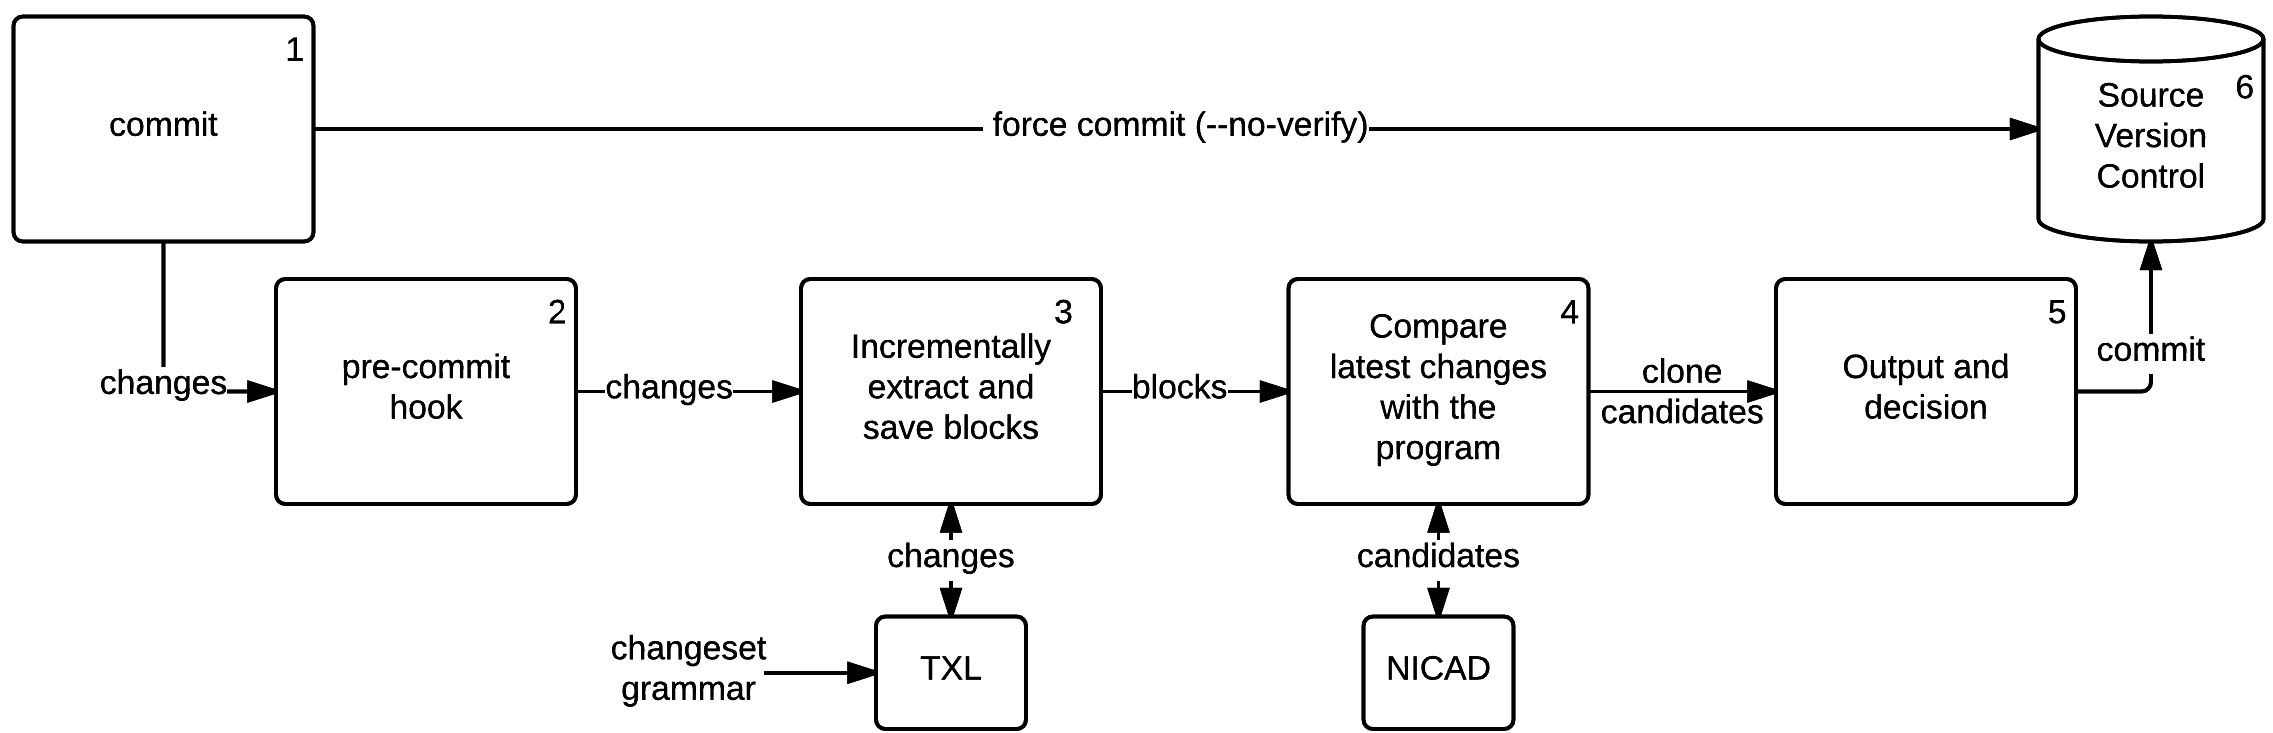
\includegraphics[width=\textwidth]{media/approach.png}
    \caption{ Overview of the PRECINCT Approach.\label{fig:precinct-approach}}
\end{figure*}

In this section, we present the PRECINCT approach and its steps in details. Our approach is composed of six different steps.
The first and the last steps are part of the day-to-day workflow of a programmer using a source version control.
Indeed the first step is the commit step where developers send their latest change to the central repository and the last step is the reception of said commit by the central repository.
The second step is the pre-commit hook which kicks in as the first operation when one wants to commit.
The pre-commit hook have access to the changes in terms of files that has been modified and more specifically, lines that has been modified.
The modified lines of the files are sent to TXL\cite{Cordy2006a} for block extraction.
Then, the blocks are compared to previously extracted blocks in order to identify clones candidates using NICAD\cite{Cordy2011}.
Finally, the output of Nicad is further refined and presented to the user for a decision round.

In the rest of this section, we present each step in details.

\subsection{Commit}
\label{sub:Commit}

In version control systems, a commit adds the latest changes to the source code to the repository, making these changes part of the head revision of the repository.
Unlike commits in data management, commits in version control systems are kept in the repository indefinitely.
Thus, when other users do an update or a checkout from the repository, they will receive the latest committed version, unless they specify they wish to retrieve a previous version of the source code in the repository.
Version control systems allow rolling back to previous versions easily. In this context, a commit within a version control system is protected as it is easily rolled back, even after the commit has been done.

\subsection{Pre-Commit Hook}
\label{sub:Pre-Commit Hook}

Hooks are custom scripts set to fire off when certain important actions occur.
There are two groups of these hooks: client-side and server-side.
Client-side hooks are triggered by operations such as committing and merging, while server-side hooks run on network operations such as receiving pushed commits.
You can use these hooks for all sorts of reasons.

The pre-commit hook is run first, before you even type in a commit message.
It's used to inspect the snapshot that's about to be committed, to see if you've forgotten something, to make sure tests run, or to examine whatever you need to inspect in the code.
Exiting non-zero from this hook aborts the commit, although you can bypass it with git commit --no-verify.
You can do things like check for code style (run lint or something equivalent), check for trailing whitespace (the default hook does exactly this), or check for appropriate documentation on new methods.

PRECINCT implementation is a suite of bash scripts and the entry point of these scripts lies in the pre-commit hooks.
Pre-commit hooks are easy to create and implement as depicted in Listing~\ref{gitprehook}.
This pre-hook is shipped with Git\footnote{https://git-scm.com/} which is a free and open source distributed version control system designed to handle everything from small to very large projects with speed and efficiency.
From lines 3 to 11, the script identifies if the commit is the first one in order to select the revision to work against.
Then, in lines 18 and 19, the script checks for trailing whitespace and fails if any are found.

\noindent\begin{minipage}{0.90\linewidth}

  \lstinputlisting[language=Bash, firstnumber=1, numbers=right, stepnumber=1,leftmargin=30, label=gitprehook, caption=Git Pre-Commit Hook Sample]{media/pre-commit.sample}

\end{minipage}

For PRECINCT to work, we just have to add the call to our script suite instead or in addition of the whitespace check.

\subsection{Extract and Save Blocks}
\label{sub:Extract and Save Blocks}

A block is a set of consecutive lines of code that will be compared to all other blocks in order to identify clones.
To achieve this critical part, we rely on TXL\cite{Cordy2006a} which is a well-known first-order functional programming over linear term rewriting.
For TXL to work, one has to write a grammar describing the syntax of the source  language and the wanted transformations.
TXL has three main phases: \textit{parse, transform}, \textit{unparse}.
In the parse phase, the grammar is controlling not only the input but also the output form. Indeed, Listing~\ref{txlsample} --- extracted from the official documentation\footnote{http://txl.ca} --- shows a grammar matching a \textit{if-then-else} statement in C with some special keywords: [IN] (indent), [EX] (exdent) and [NL] (newline) that will be used for the output form.

\noindent\begin{minipage}{0.90\linewidth}

  \lstinputlisting[language=Bash, firstnumber=1, numbers=right, stepnumber=1,leftmargin=30, label=txlsample, caption=Txl Sample Sample]{media/txl.sample}

\end{minipage}

Then, the \textit{transform} phase will, as its name suggests, apply transformation rules that can, for example, normalize or abstract the source code.
Finally, on the third phase of TXL,  called \textit{unparse}, unparses the transformed parsed input in order to output it.

Also, TXL supports what they creators calls Agile Parsing\cite{Dean}, which allow developer to redefined rule of the grammar and therefore, apply different rules than the original ones.

In PRECINCT we took advantage of that by redefining which blocks should be extracted from clone comparison and which blocks are out of scope in an effort to reduce the size (1) and ease the understandability of the output (2).

More specifically, at before each commit, we only extract the blocks belonging to the modified parts of the source code, henceforth greatly reducing the output size.

Algorithm~\ref{alg:extract} presents an overview of the extract and save blocks operation.

\begin{algorithm}[H]
 \KwData{$File[]$ modified\_files\;
 $Block[]$ prior\_blocks\;
 $Boolean$ compare\_history\;
 }
 \KwResult{Up to date blocks of the systems}
 \For{$i \leftarrow 0$ \KwTo$size\_of modified\_files$}{
    Block[] blocks $\leftarrow$ extract blocks in modified code\;
    \For{$j \leftarrow 0$ \KwTo$size\_of blocks$}{
       \If{not $compare\_history$ AND $blocks[j]$ overrides one of $prior\_blocks$}{
          delete $prior\_block$\;
       }
       write $blocks[j]$\;
    }
 }
 \caption{Overview of the Extract Blocks Operation\label{alg:extract}}
\end{algorithm}

This algorithm receives as arguments, the files that have been modified, the blocks that have been previously extracted and a boolean named compare\_history.
Then, from lines 1 to 9 lies of $for$ loop that iterates over all the modified files.
For each file (lines 2), we extract the blocks --- using TXL --- that have been modified. Then, for each extracted block, we check if the current block overrides (replace) a previous block (line 4).
In such a case, we delete the previous block as it does not represent the current version of the program anymore (line 5).
Also, we got an optional behavior of PRECINCT defined in line 4.
Indeed, the compare\_history is a condition to delete overridden blocks.
We believe that overridden blocks have been so for a good reason (bug, default, removed features, \ldots) and if a newly inserted block matches an old one, it could be worth knowing to improve the quality of the system at hand.
This feature is deactivated by default.

In summary, this step receives the files and lines modified by the latest changes of a developer and produce an up to date block representation of the system at hand.
The blocks can be analyzed in the next step to discover potential clones.

\subsection{Compare Extracted Blocks}
\label{sub:Compare Extracted Blocks}




\section{Experimentations}
\label{sec:Experimentations}

\section{Conclusion}
\label{sec:Conclusion}







\bibliographystyle{IEEEtran}
\bibliography{library.bib}


\end{document}
